\section{Introduction}\label{sec:introduction}
The structure of small-scale objects, such as a DNA molecule, is important to know, in order to understand many of their features.
The main challenge in measuring those characteristics is that some of them are too small for the equipment we currently have to detect.
One method used to overcome this obstacle is light diffraction and the unique patterns it creates when encountering such objects.
In this article we'll demonstrate some of the main features of light diffraction and how they can be used to infer the shape and size of 2-D objects, we will focus on a helix.
The helix will approximate the DNA molecule which is essentially a double helix and whose diffraction pattern can be seen in Figure~\ref{fig:Single double DNA}.
\begin{figure}[H]
    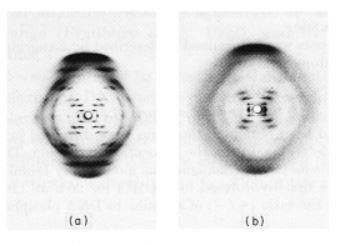
\includegraphics[width=1\columnwidth]{figures/DNA diffraction.PNG}
    \caption{Diffraction patterns of DNA complexes}
    \label{fig:DNA diffraction}
\end{figure}




